% !TEX program = pdflatex+makeindex+bibtex
% !TEX encoding = UTF-8 Unicodede_ch

% created by Simon Schälli <simon.schaelli@kantiwattwil.ch>
% v1.0 ursprüngliche Version
% v1.1 2015-10-22 mit Titelbild
% v1.2 2016-09-30 aufgeräumt
% v1.3 2016-10-16 Layoutfehler behoben

%======================================================================%
%=== Dokument auf häufige Fehler überprüfen                         ===%
%======================================================================%
\RequirePackage[l2tabu, orthodox]{nag}

%======================================================================%
%=== Dokumentklasse wählen                                          ===%
%======================================================================%
\documentclass[a4paper,openright]{scrreprt}

%======================================================================%
%=== Pakete einbinden                                               ===%
%======================================================================%
\usepackage[utf8]{inputenc}
\usepackage[english]{babel}

% Latin Modern Schriftart
\usepackage{lmodern}
\usepackage[T1]{fontenc}

% Mathematik-Pakete
\usepackage{amsmath}
\usepackage{amssymb}
\usepackage[mathscr]{euscript}

% mathematische Buchstaben als Text
\usepackage{textcomp}

% komfortable Referenzen mit \fref
\usepackage[english]{fancyref}

% Kopf- und Fusszeilen
\usepackage[automark,headsepline]{scrpage2}
\ihead[]{\headmark}
\chead[]{}
\ohead[]{\pagemark}
\ifoot[]{}
\cfoot[\pagemark]{}
\ofoot[]{}
\pagestyle{scrheadings}

% Einfügen von Bildern¨
\usepackage{float}
\usepackage{graphicx}
\usepackage{subfig}

% schöne Tabellen
\usepackage{booktabs}

% Tabelleninhalt an Dezimalpunkt ausrichten
\usepackage{dcolumn}
\makeatletter                     % <- hebt Sonderbedeutung von @ auf
\newcolumntype{d}[1]{D{.}{.}{#1}} % <- definiert einen neuen Spaltentyp
\makeatother                      % <- setzt Sonderbedeutung von @ wieder

% Algorithms
\usepackage[ruled,vlined]{algorithm2e}

% Beispieltext
\usepackage{lipsum}

% Hyperlinks in PDF
\usepackage{hyperref}

% Biblatex
\usepackage[
backend=biber,
style=numeric,
sorting=ynt
]{biblatex}
\addbibresource{Bibliography.bib}

% Macros
\usepackage{mymacros}
\usepackage{xargs}

%======================================================================%
%=== Angaben zum Dokument                                           ===%
%======================================================================%

\titlehead{Kantonsschule im Lee \hfill Kalani Fin Kistler\\
Fachschaft Mathematik \hfill Dättnauerstrasse 107\\
Rychenbergstrasse \hfill 8406 Winterthur\\
8400 Winterthur}
\subject{Matura Thesis 20/21}
\title{%
    Machines Self Teaching Soccer \\
  \large Reinforcement Learning using Policy Gradient Methods}
\author{\texorpdfstring{Kalani Fin Kistler 4h \\[1cm]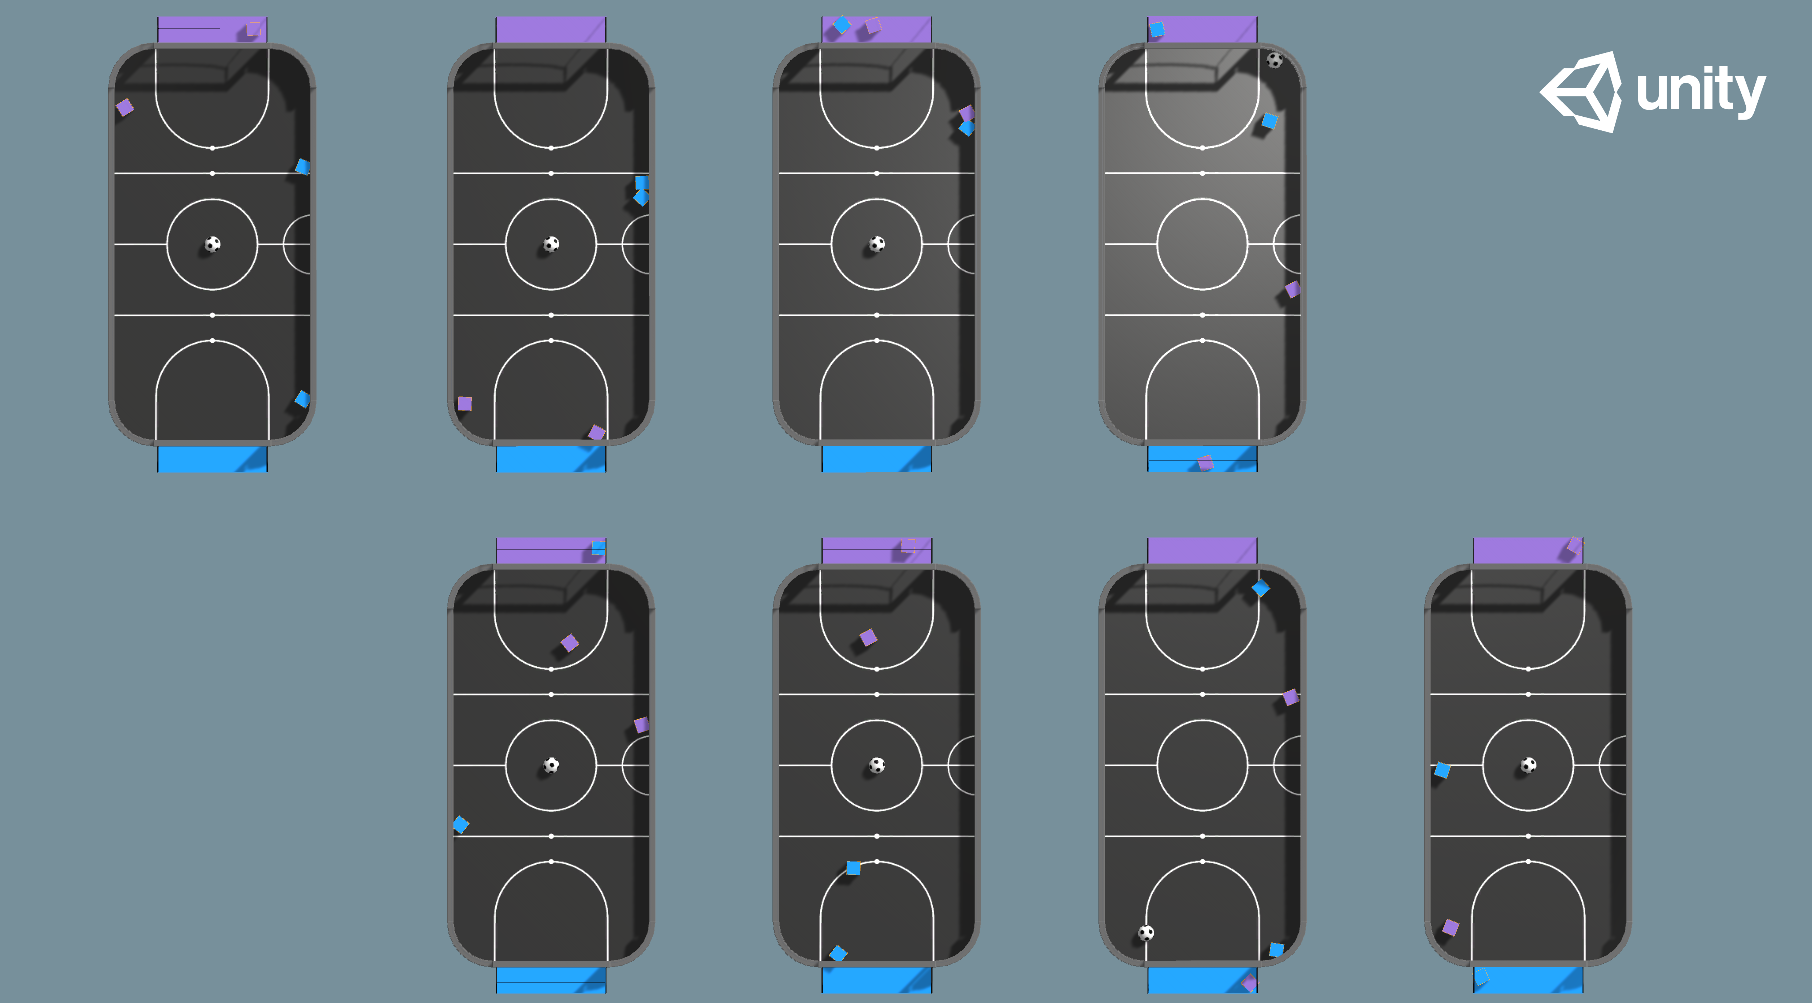
\includegraphics[scale=0.2]{figures/Screenshot from 2020-09-22 23-05-59.png}\\[1cm] {\small Supervisor: Elena Fattorini}}{Kalani Fin Kistler 4h}}
\date{\small 04.01.2021}
%======================================================================%
%=== PDF Dokumenteinstellungen                                      ===%
%======================================================================%

\makeatletter
\hypersetup{
	pdftitle={\@title},%
	pdfsubject={\@subject},%
	pdfauthor={\@author},%
	pdfkeywords={},%
	colorlinks,%
	citecolor=black,%
	filecolor=black,%
	linkcolor=black,%
	urlcolor=black}%
\makeatother
\usepackage[bottom=80pt]{geometry}


%======================================================================%
%=== Beginn des eigentlichen Dokumentes                             ===%
%======================================================================%

\begin{document}

\maketitle % <- Titel setzen
\cleardoublepage
\pagenumbering{roman} % <- römische Seitennummerierung
\tableofcontents % <- Inhaltsverzeichnis
\cleardoublepage % <- neue Seite
\pagenumbering{arabic} % <- arabische Seitennummerierung

% Kapitel einbinden:

\chapter*{NOTES FOR CHAPTER HAND IN ONLY, NOT ON FINAL}
Due to the fact that I am not yet familiar with vector graphics and wanted to focus on writing, the figures are temporary stand ins, meant only to convey the content of the final image, and are not the final images themselves.

% !TEX root = ../maturaarbeit.tex
\chapter{Introduction}\label{chap:einleitung}

% !TEX root = ../maturaarbeit.tex
\chapter{Core concepts of Reinforcement Learning}\label{chap:theory}
\section{What is Reinforcement Learning?}\label{sec:RL}
\noindent
Throughout our daily lives we navigate our surroundings, handle social situations and tackle complex tasks. In doing, so we take the actions we believe, based on experience and intuition, to have the best outcome. We might take these abilities for granted, given how natural they are to us. However, at some point we had to obtain these skills so essential in managing our day to day, many through simple trial and error. Reinforcement Learning (RL) seeks to formalize the process of figuring out how to behave based on what produces desirable results and what does not, and adjusting our future actions accordingly. 

\noindent
\\ Reinforcement Learning is a discipline of machine learning \cite[p. 1]{sutton_reinforcement_2018}, an incredibly broad field which is focused on the optimization of computer algorithms by processing data and experience. As such it is an intersection between the natural, to us intuitive concept of learning, and the rigid and numerical world of computer programming and mathematics \cite[p. 4]{sutton_reinforcement_2018}. To be able to understand how this learning process works, and to be able to quantify and formalize it, it is essential to introduce some general concepts. 

\subsection{Illustrative Example: Card game UNO}\label{subsec:UNO}

\begin{figure}[ht]
    \centering
    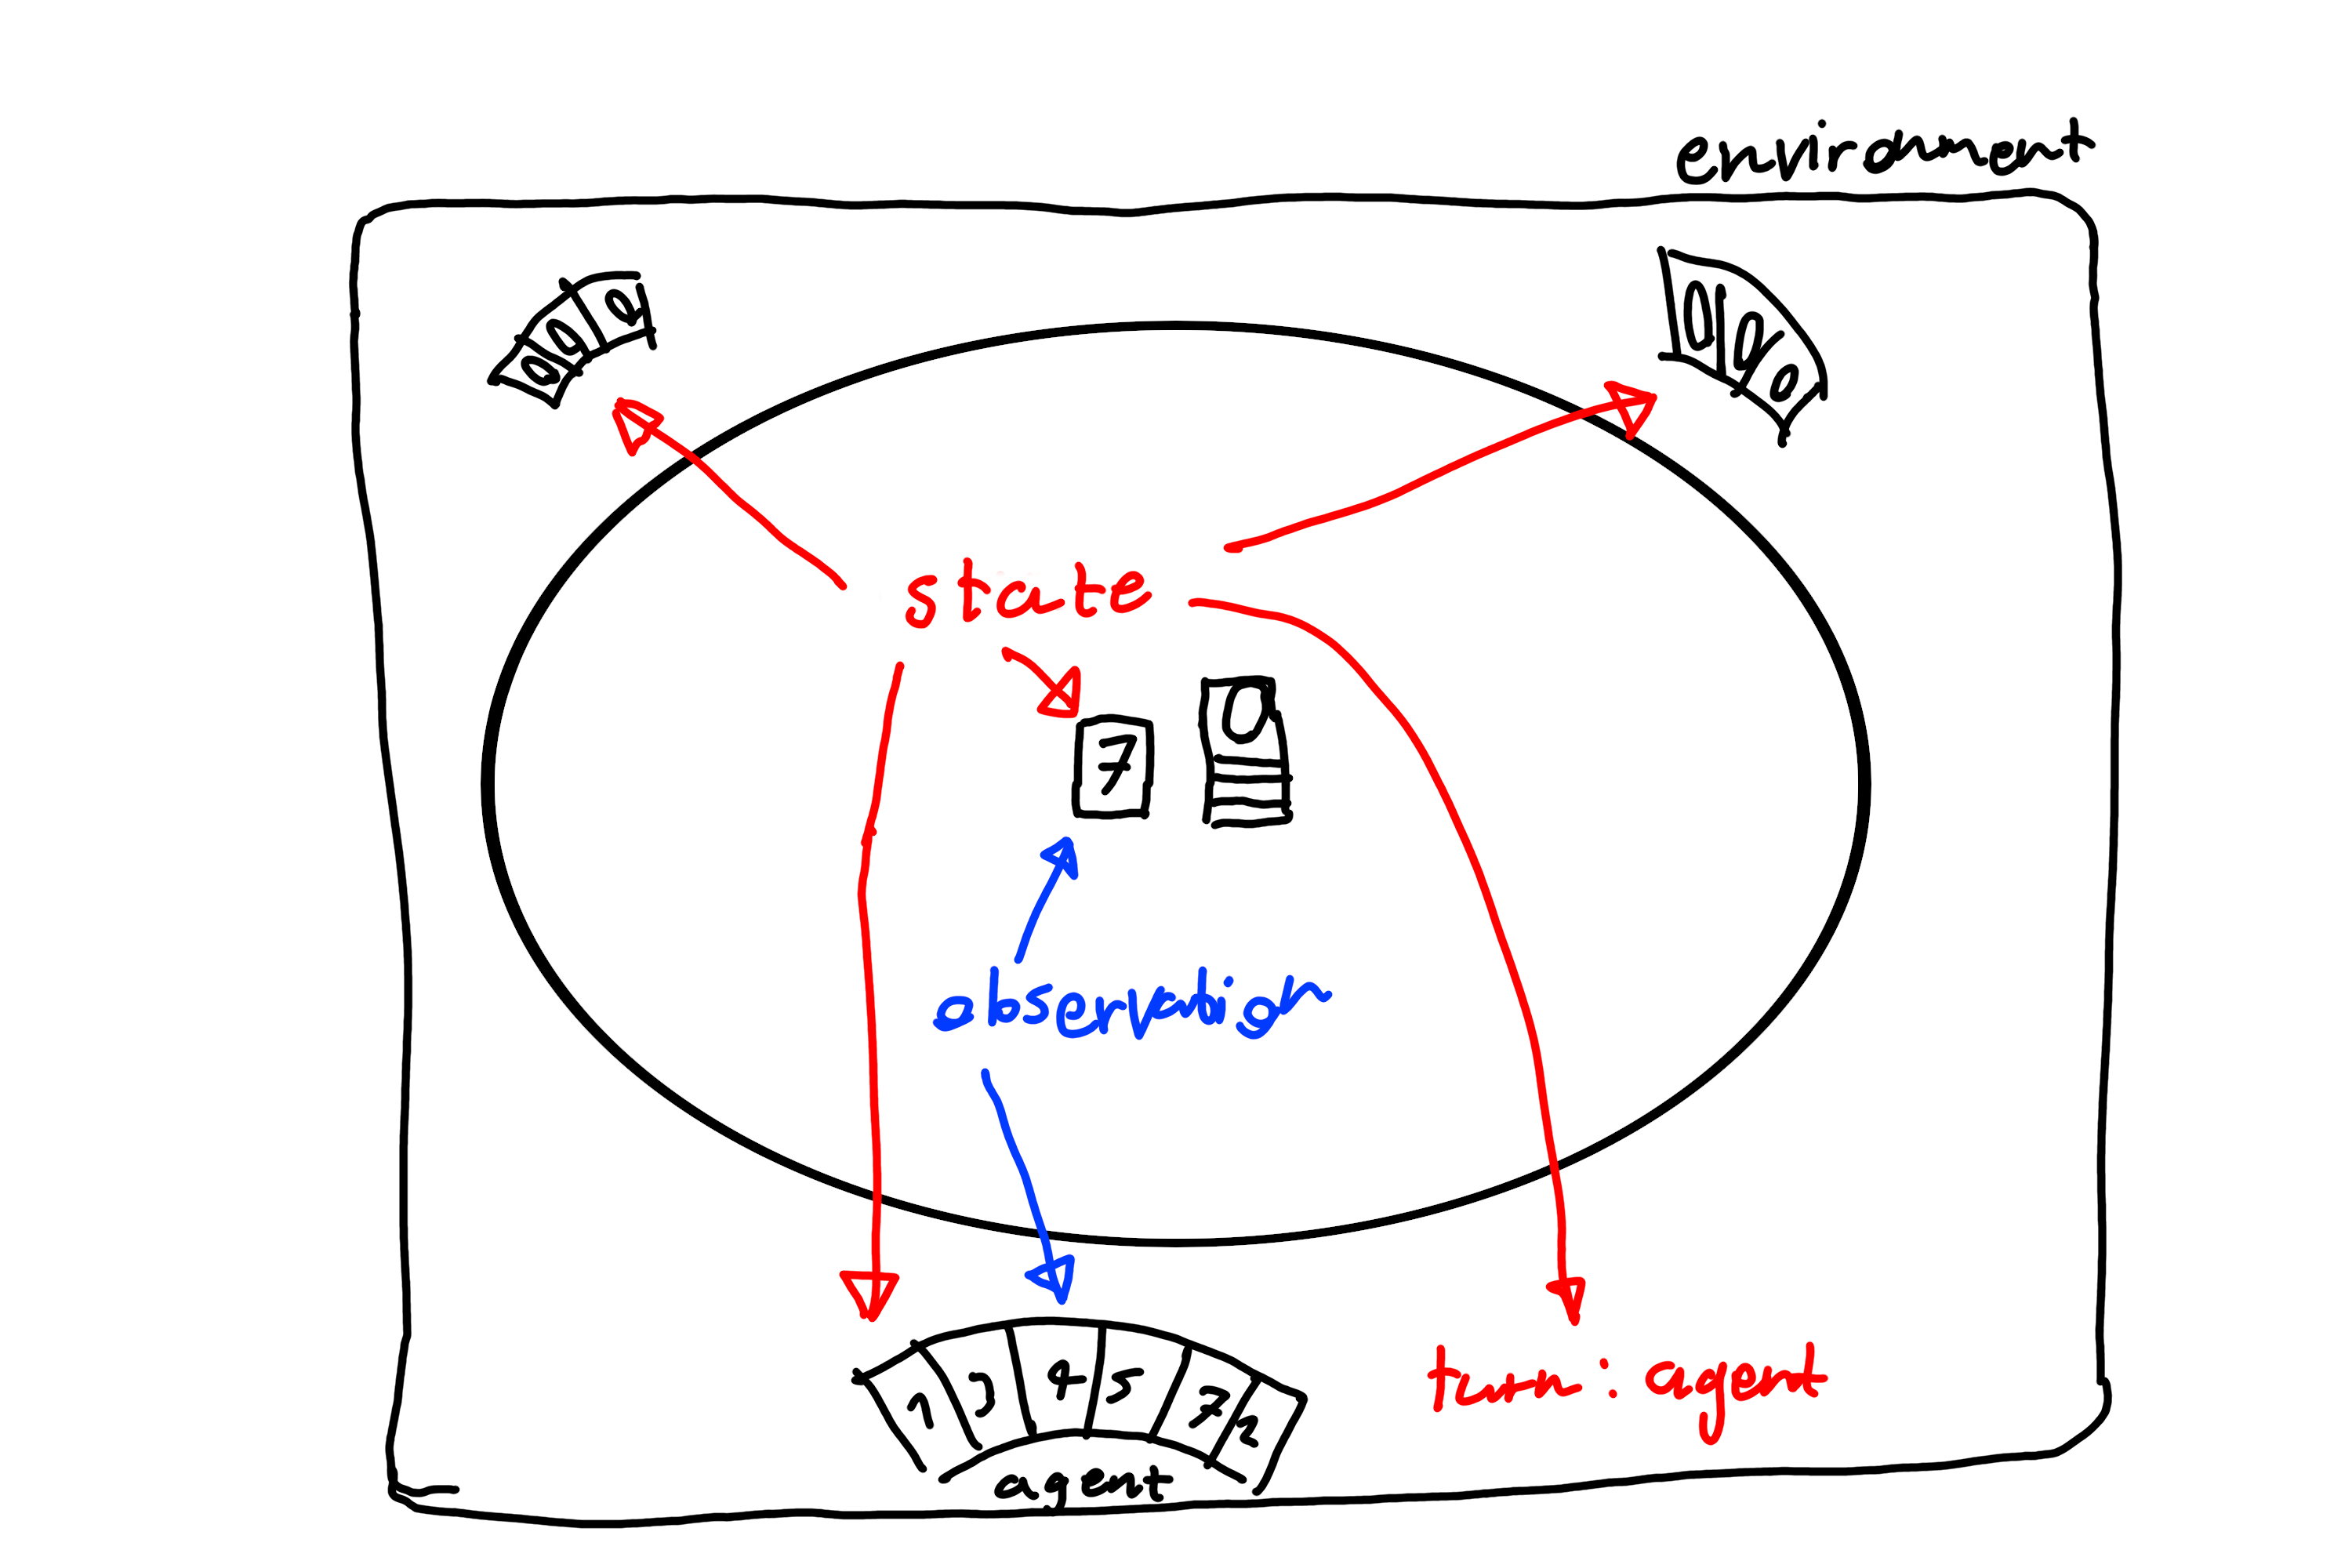
\includegraphics[width=\linewidth]{figures/UNO.png}
    \caption{UNO environment in the context of RL}
    \label{fig:UNO}
\end{figure}

\noindent
Consider the example of teaching someone how to play the popular card game “UNO”. The \textit{objective} of the game is to get rid of the cards on your hand before the other players. We can call the game an \textit{environment}. This environment contains all the players players, including their strategies, the cards and what rules the game follows. A state of an environment describes the arrangement of all components encompassed by it, in this case the hands of the players, who's turn it is, what cards are on which pile and their order. Notice that the environment contains a lot of information which the player, in Reinforcement Learning called an \textit{agent} (an actor in the environment) does not know. However, the actor can \textit{observe} the environment and thereby gain a reasonably accurate representation of it’s state. Suppose it is the agent's turn. Based on its \textit{observation} the agent can take an \textit{action a}, playing any of the cards on its hand, or picking one up. The rules of an environment might forbid certain actions, taking one of them, will lead to the same environment state, where it is the agents turn. A well designed environment will give the agent negative feedback, when teaching someone UNO, that might be telling them they did something wrong. In Reinforcement Learning this is called \textit{reward signal}. Based on the \textit{reward}, the agent then can update its behaviour to produce a different action next time. Thereby the reward \textit{reinforces} the desired behaviour, it is a \textit{reinforcement} the agent learns from. The way of acting of an agent in a state given, an observation of that state, is called a \textit{policy}, commonly denoted as $\pi$. The agent follows a policy to decide on an action, based on a state.
\newline
For the sake of brevity, unless the distinction is relevant, I am going to use the terms observation and state interchangeably. Much more expansive definitions going in to the nuances of these concepts can be found in the book \textit{Reinforcement Learning, An introduction} by Richard Sutton and Andrew Barto. \cite{sutton_reinforcement_2018}

\subsection{What Type of Problem does Reinforcement Learning suit?}\label{subsec:Why_RL}
When solving a problem where the environments rules are well known like UNO Reinforcement Learning might indeed not be the best approach. In the case of UNO, it might be more efficient to design an algorithm which computes some probability of victory for each action, based on what cards have been played and then picks the optimal one. However, this approach requires knowledge of how the environment operates \cite[p. 8]{sutton_reinforcement_2018}, if for example, it was not know what happens after our turn, it would suddenly become nigh impossible to explicitly define a probability of victory for an action. Another issue that quickly arises as the environment becomes more complex, is the rapid rise in the number of its possible permutations. Accounting for all of them quickly becomes unfeasible as the environment grows more complex. Reinforcement Learning lets us generate high quality solutions in uncertain environments based on a reward signal and the goal it ultimately describes \cite[p. 03]{sutton_reinforcement_2018}. Another approach which might come to mind as an obvious solution would be to simply mimic the behaviour of an optimal, or close to optimal, agent. However, this again is impractical as such an agent might simply not exist or generating sufficient examples can be tedious. As stated in Reinforcement Learning, An Introduction: “In uncharted territory—where one would expect learning to be most beneficial, an agent must be able to learn from its own experience.” \cite[p. 02]{sutton_reinforcement_2018} Here it is important to keep in mind that machines see environments differently from humans. For a human the actions involved in pouring a coffee, might be to pick up the can and tilt it. Plenty of examples exist on how to do that. However, we are only able to make sense of the example because we intuitively understand how move our limbs, the instructions of "pick up and tilt" would be useless to a robot which views the world through a grid of pixels and which can take only take actions in the form of powering a series of motors which move an arm, it would need an example which matches its way of interaction with the environment.

\section{The Finite Markov Decision Processes, a mathematical framework for Reinforcement Learning}\label{sec:MDP} % NOTE: THESE ARE ALL REFERENCES TO THE BOOK
I this section I will introduce Finite Markov Decision Processes (MDPs) which serve as a formalization of sequential decision making. Problems which can be described as a finite MDP are what Reinforcement Learning is trying to solve. They are called finite because the sets $\mathset{S}, \mathset{A}, \mathset{R}$ of all states, actions, and rewards respectively, are all finite. I will illustrate and apply the concepts in this section using a Grid-World environment. It serves as a particularly convenient example since in it, the state of the environment is fully described by the agent's position. This allows for simple computation and visualization. 

\subsection{Sequential decision making}\label{subsec:sequential_decision_making}
In an MDP the agent and environment continually interact. At each time step $t$ of that interaction, the agent selects an action, the environment transitions in to a new state $S_{t+1}$ and gives the reward $R_{t+1}$. Based on this new state, the agent selects another action. This series of interactions may go on forever. From this there also follows that states can be revisited, a finite set of states could not support an infinite series of transitions otherwise. $S_ {t+1}$ is just the state which the environment transitions to next and does not refer to a specific state in the set of states, the environment may even transition back to itself, in that case $S_t$ and $S_{t+1}$ would be identical. This is possible because all possible futures solely depend on that state, else it would not fully describe the environment.

\begin{figure}[h!]
    \centering
    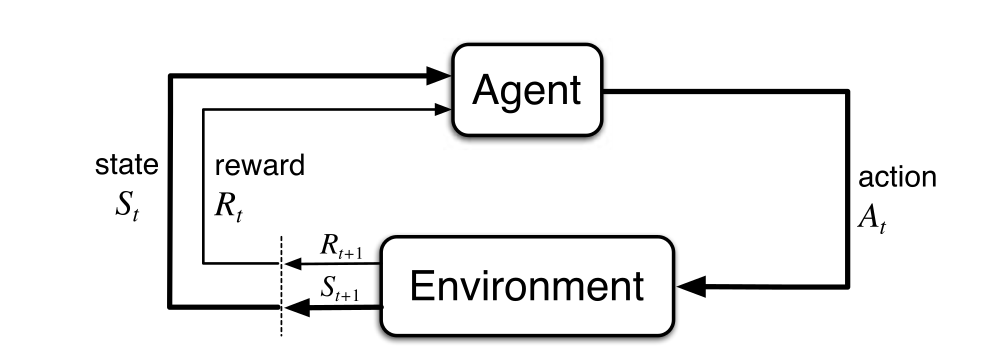
\includegraphics[width=0.7\linewidth]{figures/agent_environment_interaction_loop.png}
    \caption{Agent Environment Interaction Loop as presented in \citepg{48}}
    \label{fig:agent_env_inter}
\end{figure}

\noindent
Since the agent environment interaction is sequential, a sequence, or in Reinforcement Learning \textit{trajectory} $\tau$, arises. \citepg{48}

\begin{equation}\label{MDP:trajectory}
    \Tau = S_0, A_0, R_1, S_1, A_1, R_2 \dots
\end{equation}
\centerline{\small\textit{from \citepg{48}}}

\noindent
\\ In an \ita{episodic} environment, an environment that ends at some terminal time-step $T$, a trajectory has a terminal state $S_T$ and reward $R_T$. The notion of a terminal action does not make sense since the environment terminates at $T$, any action taken would not have an effect, and the action which proceeds $S_T$ is $A_{T-1}$.

\subsubsection{Illustrating in Grid-World}\label{subsubsec:grid_world_trajectory}
The Agent starts at a starting position, here the bottom left corner, and has to reach the upper right corner, by choosing from the actions up, down, left, right at each time step. The blacked out fields are inaccessible, running in to them or the walls, just results in the same state, the agent does not move. The rewards are not yet displayed here to avoid clutter, they will be discussed in the next section.

\begin{figure}[h!]
    \centering
    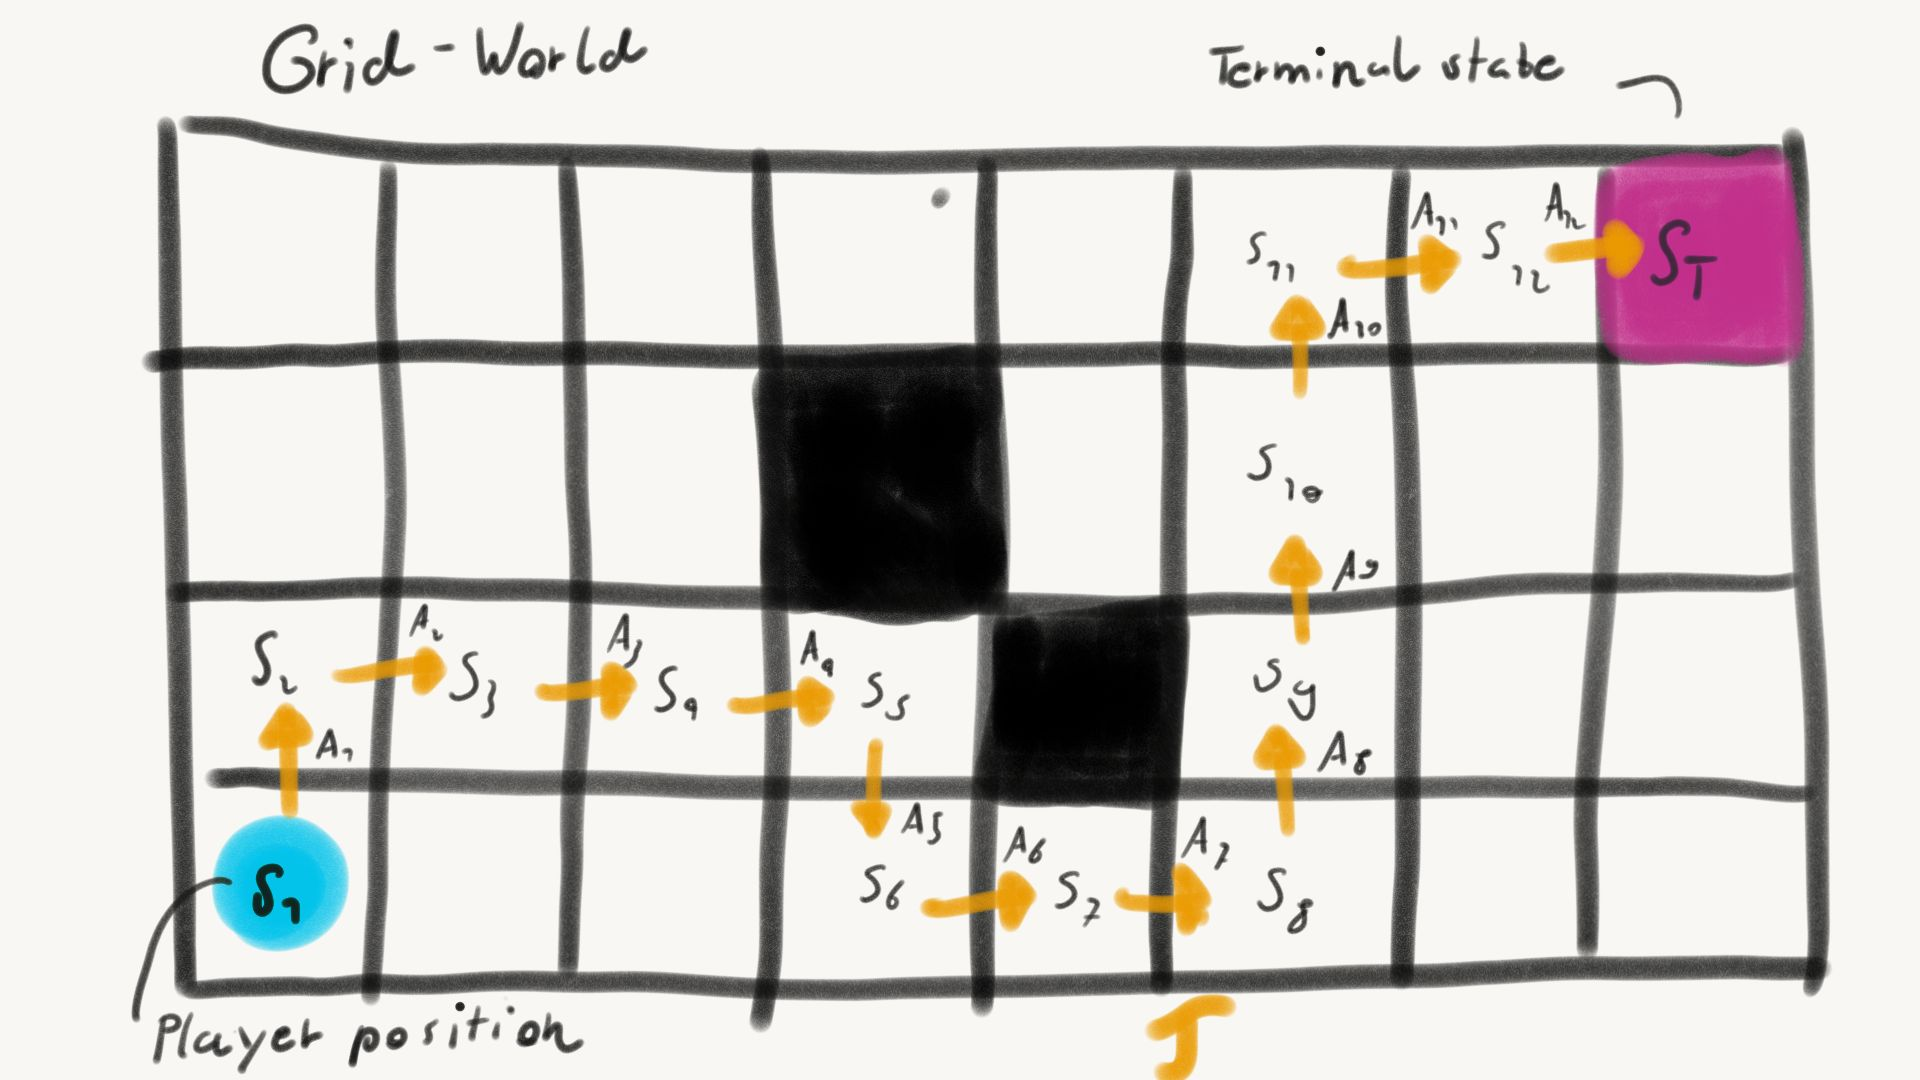
\includegraphics[width=0.7\linewidth]{figures/Grid_world_trajectory.jpeg}
    \caption{The Grid World Environment}
    \label{fig:grid_world}
\end{figure}

\noindent
The agent then moves through the states and therein generates a trajectory. The representation of that trajectory overlaid on to the grid, works in this case because the agents position fully describes an environment state. Archiving an agents trajectory becomes useful when evaluating and training the agent, since an evaluation based upon a series of correlated events, is obviously more meaningful, than one based entirely on one singular action and its consequence.

\subsection{Agent Policies in a MDP}\label{subsec:policies}

Moving forward it is important to understand what policies are mathematically. So far it has been established that policies are the way in which an chooses an action based on a state. Policies do not have to be deterministic. Mathematically, the policy is a function which takes a state and produces a probability distribution over the set of actions. This function can be parameterized, the parameter vecotr is commonly written as $\theta$. This distribution can be discrete or continuous and may produce vector actions. An action can be obtained from a policy by sampling from it. This is outlined in \citepg{58}, where $\pi(a|s)$ is defined as the probability of $a$ given $s$ under $\pi$. In our example of grid world the policy would be a discrete distribution. If the policy is parameterized, then $\pi(a|s)$ becomes $\pi(a|s,\theta)$. 

\subsection{The episodes Return, an improved measure of agent performance}\label{subsec:goals}

The agent selects actions based on state information and and receives rewards as feedback for its previous action. The goal of the agent is to maximize the reward signal received. It does that by updating its policy to produce a better action $A_t$ in the state $S_t$ based on the signal received at $t$. This means that one of the ways in which we can improve learning performance is to tweak the reward signal. The perhaps most obvious signal to give the agent is the reward $R_{t+1}$ which followed its action. However this does not take in to account any of the future states and rewards the agent's action lead to, it would not at all plan for any future states and rewards. To curb this issue we introduce the \textit{return} $G_t$. In contrast to the reward, the return also considers the influence of $A_t$ on future rewards. It is defined as follows:

\begin{equation}\label{MDP:return}
    G_t \doteq R_t + R_{t+1} + R_{t+2} \dots + R_T
\end{equation}
\centerline{\small{\ita{\citepg{54}}}}

\noindent
\\ Although the return undoubtedly is a better measure of the "goodness" of an action than the reward and training the agent using it produces decent results, it still has some flaws. Of these the most relevant to my work is that taking the sum of the rewards from the current time step to the episode's end gives the same weight to all the rewards. In many environments $A_{t-600}$ is much less relevant to $R_{t+1}$ then $A_t$, yet $R_{t+1}$ has the same weight in $G_{t}$ as it has in $G_{t-600}$. To address this, the discounted return can be used. 

\begin{equation}\label{MDP:discounted_return}
    G_t = \sum_{k=t}^{T} R_{t+k+1} \cdot \gamma ^k 
\end{equation}
or recursively as
\begin{equation}\label{MDP:recursive_discounted_return}
    R_{t+1} + \gamma \cdot G_{t+2} \mathrm{\ where\ } 0 \leq \gamma \leq 1
\end{equation}
\centerline{\small{\ita{\citepg{55}}}}

\noindent
\\ By tweaking the discount factor we can balance immediate reward with future ones. It is another hyper parameter that needs to be set which affects agent performance. Discounting also enables the use of the return in continuous environments, it is why it was originally introduced and is the main reason it is presented in \cite{sutton_reinforcement_2018}. {\\ \color{red} SHOW RESULTS OF DISCOUNT FACTOR 1 VS 0.99 AND SAY THAT IT IS BAD} \\ The returns in Grid-World with different discount factors can be seen here:

\begin{figure}[h!]
    \centering
    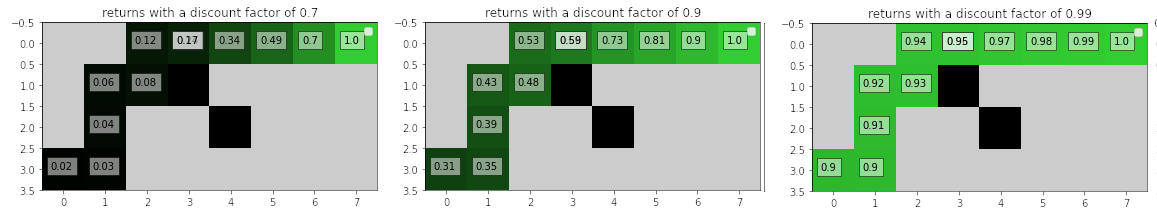
\includegraphics[width=\linewidth]{figures/grid_world_discount_factors.png}
    \caption{Returns for each time step in an episode for different discount factors}
    \label{fig:grid_world_discount_factors}
\end{figure}

\noindent
\\ The only reward the agent receives here occurs on the final time-step, and has a magnitude of 1. Notice how quickly the return decays with even a discount factor 0.9. This makes the agent quite short sighted. Due to its exponential decay small discount factors often do not make sense.

\noindent
\\ Optimizing for the return is still dependant on the quality of the rewards. Ideally, rewards should represent the thing we want the agent to achieve. Since they are the only information the agent can learn from should also not be too sparse. The problem of dealing with environments which give sparse reward is a large hurdle in modern day RL, some solutions to this are addressed in \citepg{491}. In such environments it turns out to be useful to modify the rewards received by setting baselines, creating "intrinsic rewards", those could for example be rewards for exploring the environment and many others. 

\subsection{Simple Solution for Grid-World using the presented concepts}
TODO



\chapter{Optimization with Gradient Descent}\label{gd}
All throughout Machine Learning gradient descent and variations of it are used for optimization. Gradient descent is vital for my work. As such I will I will briefly explain what it is and how it is relevant to my work.

\section{What is Gradient Descent?}\label{gd:what_is_it}
In essence gradient descent is an algorithm used to find local minima of differentiable functions. It can be thought of as starting at a point on the function graph and walking down hill until one reaches a minimum. Gradient descent works by differentiating a function at some point in order to obtain a slope, and then moving in the downwards direction of that slope. Gradient descent is done in steps. If $f(\theta)$ is a differentiable function, then one gradient descent step is:

\begin{equation}\label{Graident_Descent:basic_update}
    \theta \leftarrow \theta - \alpha \cdot \frac{\partial}{\partial \theta}f(\theta)
\end{equation}

\noindent
\\ The \textit{step size} $\alpha$ is introduced to control the magnitude of the descent step. The gradient descent algorithm consists of performing these steps iteratively until the current value (in the above case $\theta$) is sufficiently close to the actual local minimum. Performing 10 gradient descent steps on the function $f(\theta) = \theta^2$ and a starting value of $\theta = 3$ with various values for alpha looks as follows:

\begin{figure}[ht]
    \centering
    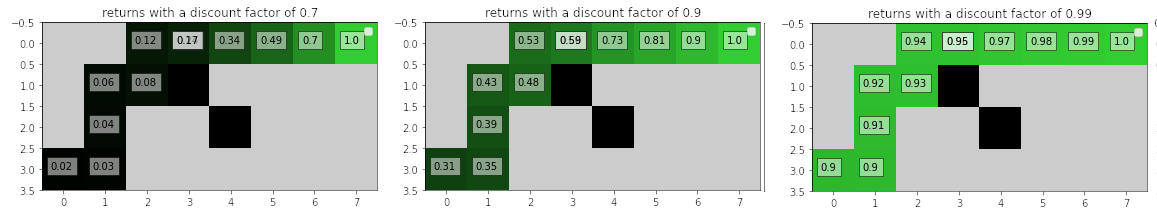
\includegraphics[width=\linewidth]{figures/grid_world_discount_factors.png}
    \caption{Gradient Descent on $f(\theta) = \theta^2$}
    \label{fig:UNO}
\end{figure}

\noindent
\\ As can be clearly seen here smaller step sizes lead to more accurate results. Too large a step size may even lead to divergence. However, if the step size is too small, it may take very long to reach a local minimum. Gradient descent functions in the exact same way if $\theta$ is a vector. In that case the update step becomes:

\begin{equation}\label{Graident_Descent:basic_update_vector}
    \theta \leftarrow \theta - \alpha \cdot \nabla_\theta f(\theta)
\end{equation}

\subsection{Gradient Descent on functions which take unknown variables}\label{gd:random_var}
Gradient Descent can also be used to minimize function parameters when unknown variables are in the mix, and the goal is to find parameters which lead to minimal function values for most parameters. Say $f(x, \theta)$ is the function we are performing gradient descent on, $\theta$ is a vector of parameters we are trying to optimize, and $x$ is sampled from a distribution. We can perform gradient descent steps which are close to optimal, by calculating the gradients $\nabla_\theta f(x, \theta)$ for $n$ number of samples of $x$, averaging them, and performing a gradient descent step on that average. The more samples of $x$ we have the more accurate the direction and magnitude of the step are going to be going to be.

\subsection*{Gradient Ascent}\label{gd:gradient_ascent}
As the name implies gradient ascent is the exact opposite of gradient descent. Instead of trying to find the local minimum of a function, when performing gradient ascent we are trying to find the local maximum of a function. Gradient Ascent is identical to performing Gradient Descent on the negative derivatives. 

\section{How is Gradient Descent relevant to Reinforcement Learning?}\label{gd:relevance}
In the previous chapter we have established that policies are functions which take actions and produce probability distributions over a set of actions. They may also be parameterized. One very common way of optimizing policies is to define a function $J(\theta)$, which measures agent performance \citepg{312}. This function is dependant on, and differentiable with respect to, the policy parameters $\theta$. Gradient Descent or Ascent (which one we use is dependant on if the performance measuring function treats lower or larger values as better) can then be used to optimize $\theta$. I will present one such function, in chapter \ref{chap:policy_gradient}. Gathering a set of agent-environment interactions, using the rewards received in them in a performance measuring function which depends on the policy parameters, and then using a variation on Gradient Descent to optimize those parameters, is the method i use to train an agent in this thesis. This can be represented in an abstract algorithmic fashion:

\begin{algorithm}[H]
\SetAlgoLined
 initialization\;
 \Repeat{agent performance suffices}{
  \For{$t \in 0, \dots, n$}{
   Get state $S_t$\;
   Take action $A_t$ sampled from $\pi(a|s,\theta)$\;
   Receive reward $R_t$\;
  }
  Compute gradients of performance function based on rewards w.r.t. $\theta$\;
  update $\theta$ with Gradient Descent;
  
 }
 \caption{Reinforcement Learning With Gradient Descent}
\end{algorithm}

% !TEX root = ../maturaarbeit.tex
\newpage
\chapter{Solutions with Policy Gradient Methods: WORK IN PROGRESS}\label{chap:policy_gradient}
\noindent
In this section I shall briefly present Policy Gradient methods, their advantages and aim to give an intuitive understanding of their operation to the reader. Policy Gradients (PG) are the basis of the algorithm used in this thesis to solve the soccer problem. They are one of the main methods used in modern Reinforcement Learning. Countless algorithms build on them, one of which I will present and use here.

\section{What are Policy Gradient Methods?}\label{pg:what_are_policy_gradient_methods}
Policy Gradient Methods Rely on the concept of the policy as a function which produces a probability distribution over the action space, and the concept of gradient ascent, which i discussed in the previous chapter \ref{gd:gradient_ascent}. At the end of that chapter I mentioned how Gradient Descent / Ascent could be used in Learning, By defining a Performance Measure dependant on the policy's parameters, and then differentiating that with respect to those parameters, thereby finding out in what direction to change them in order to improve the policy. Here I will present just such a measure, denoted as $J(\theta)$. Conceptually $J(\theta)$ is the true value of of $\pi$ with the parameters $\theta$ starting in a state $s_0$. It can be thought of as a measure of how well an agent following the policy will perform starting at $s_0$. 

\section{Why I chose Policy Gradient Methods for my Work}\label{pg:reasons_for_pg}
\noindent
Regrettably the field of Reinforcement Learning is far too broad to cover all of its approaches here, and thus laying out the advantages of Policy Gradient methods over other approaches is inevitably limited by the limited context available. 

\section{The Policy Gradient Theorem}\label{pg:theorem}
In \citepg{324} $J(\theta)$ it is defined as follows:

\begin{equation}\label{pg:performance_measure}
    J(\theta) \doteq v_{\pi_\theta}(s_0)
\end{equation}
\noindent
where $v_\theta(s_0)$ is:
\begin{equation}\label{pg:true_value_function}
    v_{\pi_\theta}(s) \doteq \mathbb{E}_{\pi_\theta}[G_t|S_t=s]
\end{equation}
\centerline{\small\textit{from \citepg{58}}}

\noindent
\\ I will not be using $v_{\pi_\theta}(s)$ in my thesis, it extends beyond the scope of my work, especially as it pertains to the practical part. I bring it up here because it is used in the definition of $J(\theta)$ in the Policy Gradient Theorem \ref{pg:theorem}
% !TEX root = ../maturaarbeit.tex
\newpage
\chapter{Function approximation using Deep Neural Networks: WORK IN PROGRESS}\label{chap:neural_networks}

% !TEX root = ../maturaarbeit.tex
\printbibliography[
heading=bibintoc,
title={Bibliography}
] 

\appendix 
\listoffigures 
\listoftables 
\end{document}